\documentclass[11pt]{article}
\usepackage[margin=0.9in]{geometry}
\usepackage{amsmath}
\usepackage{booktabs}
\usepackage{graphicx}
\usepackage{float}
\usepackage{hyperref}
\usepackage{setspace}
\usepackage{hanging}

\hypersetup{colorlinks=true, linkcolor=blue, citecolor=blue, urlcolor=blue}
\setstretch{1.08}

\title{Early-Pandemic Migration-Demand Shocks and Subsequent Rent Growth}
\author{Draft}
\date{May 2026}

\begin{document}
\maketitle

\begin{abstract}
This paper studies whether counties exposed to unusually large early-pandemic migration-demand shocks experienced faster subsequent rent growth. I define a county's migration shock as its 2021 IRS net migration rate relative to its own 2019--2020 pre-pandemic baseline and classify counties into five shock quintiles. The main empirical design uses a lagged binned difference-in-differences and event-study framework with county and year fixed effects, where post-treatment rent growth begins in 2022. This design treats migration as a broad demand shock that may include population inflow, migrant composition, income, remote-work status, and housing preferences, rather than as a clean instrument for population growth. I then test whether the rent response is larger in low-permit counties, used as an imperfect proxy for supply-constrained housing markets. The identifying assumption is that high- and middle-shock counties would have followed parallel rent-growth trends absent the migration shock, which I assess using event-study pre-trends.
\end{abstract}

\section{Research Question}

The COVID-19 pandemic changed where many households could live. Remote work, demand for space, and amenity preferences allowed some households to move away from traditional employment centers and toward different local housing markets. This paper asks whether counties that experienced unusually large early-pandemic migration-demand shocks subsequently experienced faster rent growth.

The estimand is reduced form. I do not interpret the main coefficient as the pure causal effect of population growth. IRS migration shocks may bundle several mechanisms: population inflow, higher-income movers, remote-work status, demand for larger units, and willingness to pay for local amenities. The empirical question is therefore whether exposure to a large early-pandemic migration-demand shock predicts faster subsequent rent growth, and whether this relationship is stronger in counties where housing supply appears more constrained.

\section{Data}

The unit of analysis is a county-year panel. Rent outcomes come from Zillow's county-level Zillow Observed Rent Index (ZORI), aggregated from monthly observations to annual county rent levels. The outcome is annual log rent growth,
\[
\Delta \log Rent_{ct}=\log Rent_{ct}-\log Rent_{c,t-1}.
\]
Migration measures come from IRS county migration files. IRS years are interpreted as destination years; for example, the 2019--2020 file corresponds to destination year 2020. I use exemptions, which are closer to persons than tax returns, to define county net migration rates:
\[
NetMigRate_{ct}=\frac{Inflow_{ct}-Outflow_{ct}}{PopulationBase_{c,t-1}}.
\]
The population base is constructed from IRS exemptions as non-migrant exemptions plus out-migrant exemptions. The ideal supply-side measure would be a direct county-level index of zoning or land-use restrictiveness, since restrictive zoning is one institutional reason local housing supply may respond slowly to demand shocks. Such zoning measures are not consistently available for the full county sample used here. I therefore proxy for supply constraints using 2020 residential permits per capita from the Census Building Permits Survey. Counties with fewer permits per capita are treated as lower-permit, potentially more supply-constrained markets. This proxy is motivated by zoning and supply-elasticity theory, but it should not be interpreted as a direct legal zoning measure.

The analysis uses public data sources: Zillow ZORI for rents, IRS SOI county migration files for inflows and outflows, and the Census Building Permits Survey for residential permitting. A secondary extension can also merge Census county population estimates to rescale the reduced-form migration shock into measured population growth, but that exercise requires stronger assumptions and is not the main design.

\section{Treatment Timing and Empirical Design}

The treatment is based on an early-pandemic abnormal migration shock. For county $c$, define the pre-pandemic baseline as
\[
PreNetMigRate_c = 0.5(NetMigRate_{c,2019}+NetMigRate_{c,2020}),
\]
and define the early-pandemic shock as
\[
Shock_c = NetMigRate_{c,2021} - PreNetMigRate_c.
\]
The main specification divides counties into five quintiles of $Shock_c$. Q3 is the omitted middle-shock group. The post period starts after the early migration shock:
\[
Post_t=1[t\geq 2022].
\]
The main binned DiD model is
\[
\Delta \log Rent_{ct}
= \sum_{q\in\{Q1,Q2,Q4,Q5\}}\beta_q Q_{cq}\times Post_t
+\alpha_c+\delta_t+\epsilon_{ct},
\]
where $\alpha_c$ are county fixed effects and $\delta_t$ are year fixed effects. Standard errors are clustered by county.

The event-study specification focuses on the highest-shock quintile relative to Q3:
\[
\Delta \log Rent_{ct}
= \sum_{\tau\neq 2019}\theta_\tau Q5_c\times 1[t=\tau]
+\alpha_c+\delta_t+\epsilon_{ct}.
\]
The omitted year is 2019. This figure is a central diagnostic, not an appendix check.

\section{Identification}

The key identifying assumption is parallel trends: absent the early-pandemic migration-demand shock, high-shock and middle-shock counties would have followed similar rent-growth trajectories after 2021. This assumption may fail if high-shock counties were already improving in amenities or labor markets, if pandemic migrants were systematically richer or more likely to work remotely, or if regional shocks such as growth in Sun Belt markets drove both migration and rents. Rent growth itself can also affect migration if treatment and outcome windows overlap.

The revised design addresses these concerns by defining treatment using the early 2021 migration shock and measuring the main rent response beginning in 2022. County fixed effects remove time-invariant county differences, and year fixed effects remove common annual shocks. Event-study estimates assess whether rent-growth trends were already diverging before the shock. The design remains reduced form: it estimates the relationship between early migration-demand exposure and subsequent rent growth, not the pure effect of measured population counts.

\section{Results}

\subsection{Descriptive Evidence}

Table \ref{tab:shock_quantiles} reports the shock cutoffs used to form the five groups. The 80th percentile is positive, so the highest-shock quintile experienced positive abnormal net migration on average. Table \ref{tab:shock_group_summary} shows that Q5 counties had the largest average shock and the highest mean 2022--2023 rent growth, but they also had higher 2020 permits per capita. This means supply heterogeneity must be interpreted carefully.

\begin{table}[!htbp]\centering
\caption{Early-Pandemic Abnormal Migration Shock Cutoffs}\label{tab:shock_quantiles}
\begin{tabular}{lr}\toprule
Quantile & Shock cutoff \\
\midrule
P20 & -0.0034 \\
P40 & -0.0008 \\
P60 & 0.0015 \\
P80 & 0.0047 \\
\bottomrule
\end{tabular}
\end{table}

\begin{table}[!htbp]\centering
\caption{Summary Statistics by Early-Pandemic Migration-Shock Quintile}\label{tab:shock_group_summary}
\begin{tabular}{lrrrrr}\toprule
Group & Counties & Shock & 2021 net mig. rate & Rent growth & Permits pc \\
\midrule
Q1 lowest & 111 & -0.0074 & -0.0109 & 0.0644 & 0.0058 \\
Q2 & 110 & -0.0020 & -0.0041 & 0.0721 & 0.0055 \\
Q3 middle & 111 & 0.0004 & 0.0044 & 0.0763 & 0.0059 \\
Q4 & 110 & 0.0028 & 0.0058 & 0.0761 & 0.0058 \\
Q5 highest & 111 & 0.0097 & 0.0254 & 0.0823 & 0.0114 \\
\bottomrule
\multicolumn{6}{p{0.88\textwidth}}{\footnotesize Notes: Shock is the 2021 IRS net migration rate minus the county's own 2019--2020 baseline. Rent growth is mean annual log ZORI rent growth in 2022--2023. Permits pc is 2020 residential permits per IRS population base.}
\end{tabular}
\end{table}


\begin{figure}[H]
\centering
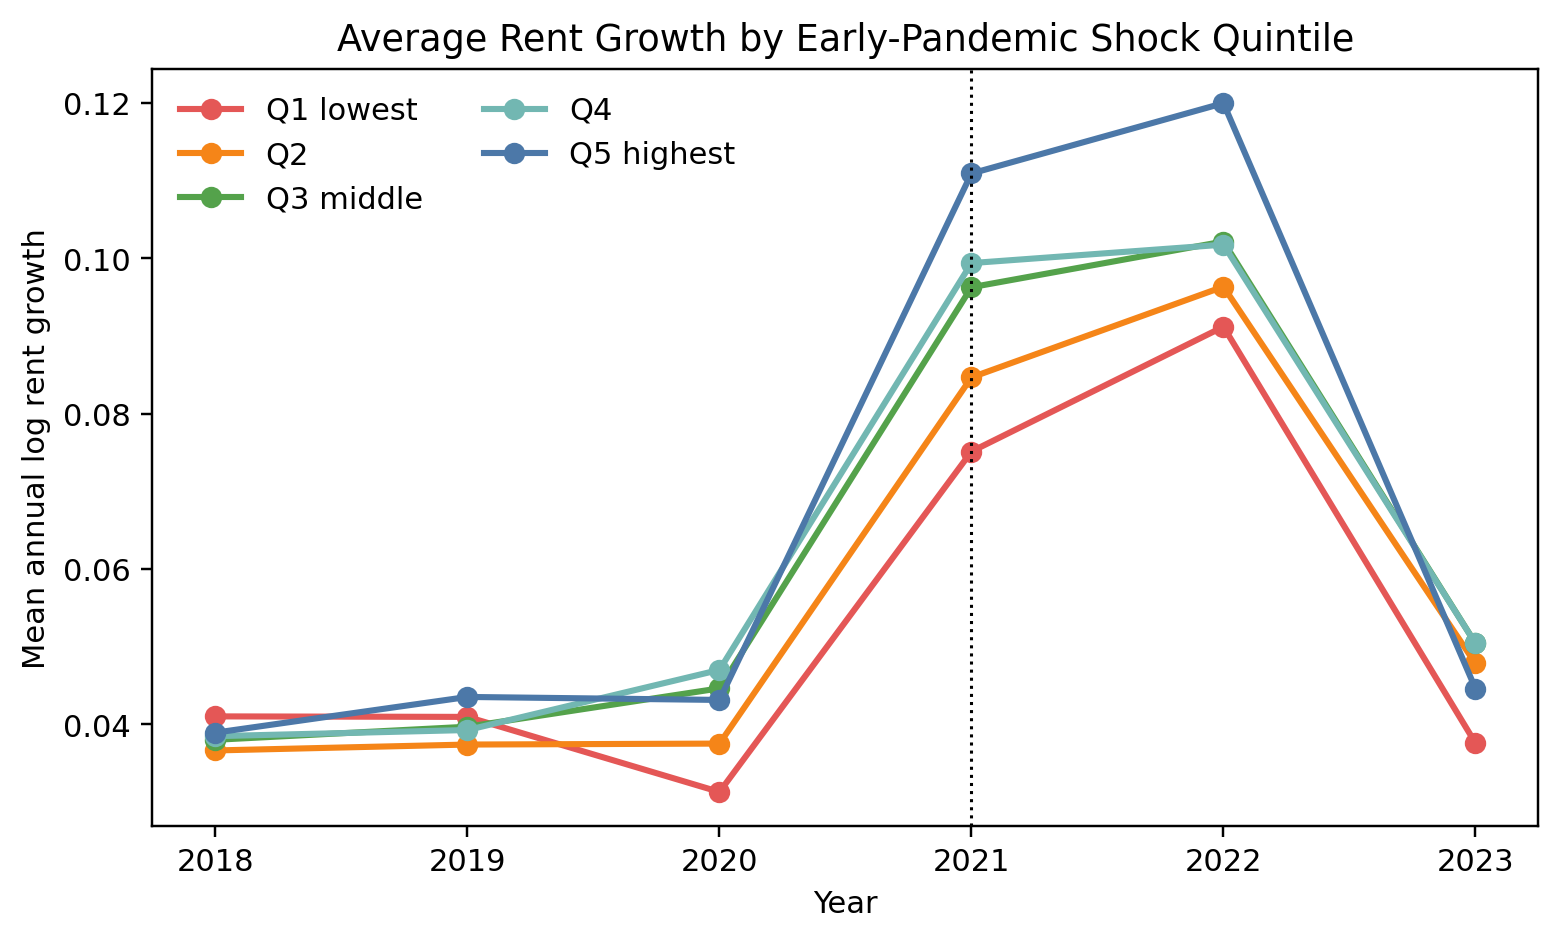
\includegraphics[width=0.78\textwidth]{../output/figures/rent_growth_by_early_shock_quintile.png}
\caption{Average Annual Rent Growth by Early-Pandemic Shock Quintile}
\label{fig:raw_trends}
\end{figure}

Figure \ref{fig:raw_trends} plots raw rent-growth trends by shock quintile. The plot is useful for checking whether the groups were moving similarly before the post period and whether separation appears after the early-pandemic shock.

\subsection{Event-Study Evidence}

\begin{figure}[H]
\centering
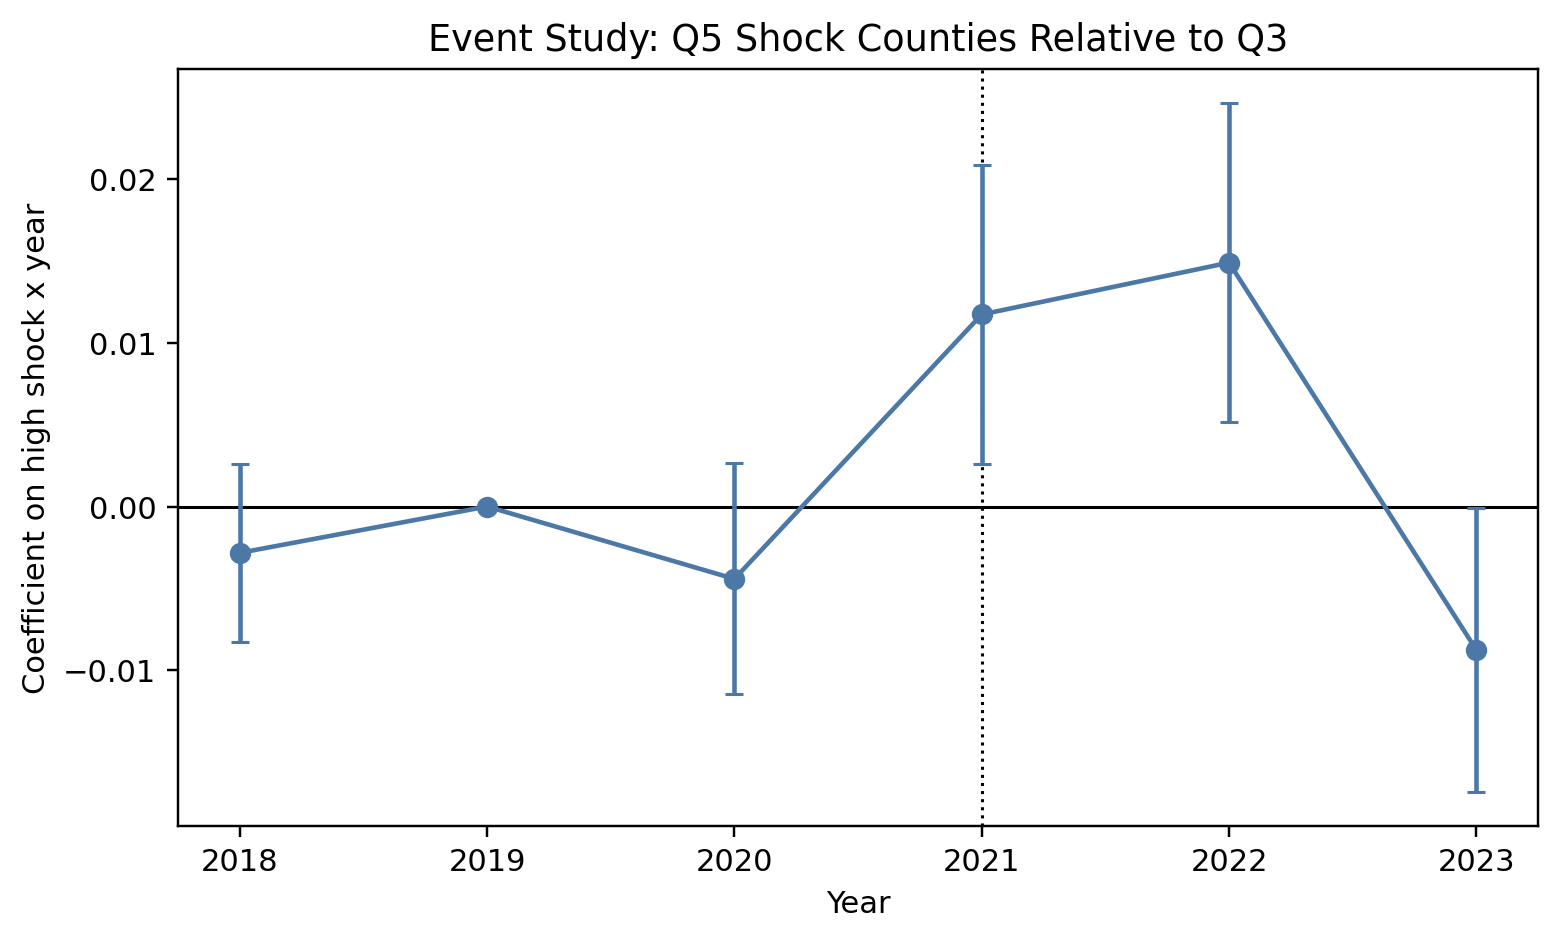
\includegraphics[width=0.78\textwidth]{../output/figures/event_study_q5_vs_q3.png}
\caption{Event-Study Coefficients: Q5 Relative to Q3}
\label{fig:event_study}
\end{figure}

Figure \ref{fig:event_study} reports event-study coefficients for Q5 counties relative to Q3 counties. The 2018 and 2020 pre/post-boundary coefficients are close to zero relative to their confidence intervals, while 2021 and 2022 are positive. The 2023 coefficient turns negative. This pattern is suggestive of a short-run post-shock rent response, but the reversal in 2023 means the evidence is not a clean monotonic treatment effect.

\subsection{Main DiD Estimate}

\begin{table}[!htbp]\centering
\caption{Lagged Five-Bin Difference-in-Differences}\label{tab:main_lagged_did}
\begin{tabular}{lc}\toprule
 & Annual log rent growth \\
\midrule
Q1 lowest shock $\times$ Post & -0.0040 \\
 & (0.0041) \\
Q2 $\times$ Post & 0.0014 \\
 & (0.0031) \\
Q4 $\times$ Post & -0.0014 \\
 & (0.0031) \\
Q5 highest shock $\times$ Post & 0.0019 \\
 & (0.0030) \\
\midrule
County fixed effects & Yes \\
Year fixed effects & Yes \\
Observations & 3,256 \\
$R^2$ & 0.675 \\
\bottomrule
\multicolumn{2}{p{0.76\textwidth}}{\footnotesize Notes: Post is 2022--2023. The reference group is Q3 middle-shock counties. Standard errors are clustered by county. Significance levels: * $p<0.10$, ** $p<0.05$, *** $p<0.01$.}
\end{tabular}
\end{table}


Table \ref{tab:main_lagged_did} shows the main lagged five-bin DiD estimates. Relative to Q3 counties, Q5 counties have a post-2021 coefficient of 0.0019 with a standard error of 0.0030. The estimate is positive but imprecise. Q1 counties have a negative coefficient, while Q2 and Q4 are close to zero. I therefore interpret the main binned evidence as suggestive but not conclusive.

\subsection{Supply-Constraint Heterogeneity}

\begin{table}[!htbp]\centering
\caption{Supply-Constraint Heterogeneity Using Low 2020 Permits}\label{tab:supply_heterogeneity}
\begin{tabular}{lc}\toprule
 & Annual log rent growth \\
\midrule
Q5 highest shock $\times$ Post & 0.0051 \\
 & (0.0038) \\
Q5 highest shock $\times$ Post $\times$ Low permit & -0.0017 \\
 & (0.0051) \\
Low permit $\times$ Post & 0.0079*** \\
 & (0.0027) \\
Q1 lowest shock $\times$ Post & -0.0036 \\
 & (0.0040) \\
\midrule
County fixed effects & Yes \\
Year fixed effects & Yes \\
Observations & 3,256 \\
$R^2$ & 0.678 \\
\bottomrule
\multicolumn{2}{p{0.76\textwidth}}{\footnotesize Notes: Low permit equals one for counties below the sample median of 2020 residential permits per capita. Standard errors are clustered by county. Significance levels: * $p<0.10$, ** $p<0.05$, *** $p<0.01$.}
\end{tabular}
\end{table}


Table \ref{tab:supply_heterogeneity} tests whether the Q5 response is larger in low-permit counties. This exercise is intended to approximate the zoning/supply-constraint mechanism: if restrictive land-use regulation or other supply frictions limit new construction, then a migration-driven demand shock should translate more strongly into rent growth. The coefficient on $Q5\times Post\times LowPermit$ is negative and imprecise. Thus, using 2020 permits per capita as the available supply proxy, I do not find strong evidence that low-permit counties experienced a larger Q5 rent-growth response. This does not rule out zoning heterogeneity; it only means that this permit-based proxy does not provide conclusive support in the current panel. A stronger test would merge a direct zoning index, such as a Wharton-style land-use regulation measure, and compare the permit-based results with legal restrictiveness measures.

\subsection{Robustness}

As robustness, I estimate a continuous-shock specification and a version excluding 2023, the year affected by IRS matching-process changes. These results are reported in the output tables and should be interpreted as sensitivity checks rather than the main design. Appendix \ref{app:iv} also discusses an IV scaling exercise that instruments measured Census population-growth shocks with IRS migration shocks. I do not use that IV as the main identification strategy because it requires the stronger exclusion restriction that IRS migration shocks affect rents only through measured population growth. Future extensions should add ACS median gross rent, population weights, state-by-year or region-by-year shocks, and direct zoning or vacancy measures.

\section{Conclusion}

This paper revises the migration-rent design around treatment timing. Counties are grouped by abnormal 2021 net migration relative to their own 2019--2020 baseline, and the main outcome is subsequent rent growth in 2022--2023. The results are mixed. Descriptive and event-study evidence show some short-run separation for the highest-shock counties, but the main five-bin DiD estimate for Q5 is positive and statistically imprecise, and the effect does not persist cleanly through 2023. The supply-constraint interaction using low 2020 permits is also imprecise.

The evidence is therefore best read as suggestive rather than definitive. The revised design is more credible than a contemporaneous cumulative 2020--2022 binning strategy, but the identifying assumption remains strong: high-shock counties must have followed similar rent-growth paths absent the early-pandemic migration-demand shock. A stronger final version would merge richer supply measures, especially direct zoning or vacancy data, and report additional state- or region-adjusted robustness checks.

\appendix

\section{IV Scaling Exercise}
\label{app:iv}

As a secondary exercise, one can use IRS migration shocks as an instrument for measured Census population-growth shocks. This exercise answers a different question from the main paper. The main design estimates the reduced-form relationship between abnormal population-inflow exposure and subsequent rent growth. The IV exercise instead rescales that relationship by measured Census population growth:
\[
Y_c = \beta D_c + X_c^{\prime}\gamma + \epsilon_c,
\]
where $Y_c$ is rent-growth acceleration, $D_c$ is a Census population-growth shock, and $D_c$ is instrumented by an IRS migration shock. In the earlier IV version of this project, the treatment was
\[
D_c = \Delta \log Pop_{c,2021:2022} - \Delta \log Pop_{c,2019:2020},
\]
the outcome was
\[
Y_c = \Delta \log Rent_{c,2021:2022} - \Delta \log Rent_{c,2019:2020},
\]
and the instrument was
\[
Z_c = IRSInflowRate_{c,2021:2022} - IRSInflowRate_{c,2019:2020}.
\]

The motivation for this exercise is intuitive: if IRS migration shocks predict actual Census population growth, the IV coefficient can be read as a population-growth-scaled rent response. The limitation is equally important. The exclusion restriction requires IRS migration shocks to affect rents only through measured population growth. That may fail during the pandemic because migrants may differ in income, remote-work status, demand for space, and willingness to pay for amenities. For that reason, I interpret the IV estimates as suggestive scaling evidence rather than definitive causal estimates.

\begin{table}[H]\centering
\caption{Appendix: IV Scaling Estimates from Earlier Specification}
\label{tab:iv_appendix}
\begin{tabular}{lrrrrr}
\toprule
Specification & Estimate & Std. error & 95\% CI low & 95\% CI high & First-stage F \\
\midrule
No controls & 3.433 & 1.524 & 0.446 & 6.420 & 9.113 \\
Baseline controls & 2.330 & 0.947 & 0.473 & 4.187 & 13.514 \\
Controls + state FE & 0.599 & 0.568 & -0.514 & 1.712 & 5.660 \\
\bottomrule
\multicolumn{6}{p{0.88\textwidth}}{\footnotesize Notes: The endogenous treatment is a Census population-growth shock; the instrument is an IRS migration shock. The estimates come from the earlier IV version of the project and are reported here only as a scaling exercise.}
\end{tabular}
\end{table}

\begin{table}[H]\centering
\caption{Appendix: IV Supply-Constraint Split from Earlier Specification}
\label{tab:iv_supply_appendix}
\begin{tabular}{lrrrrr}
\toprule
Group & Estimate & Std. error & 95\% CI low & 95\% CI high & First-stage F \\
\midrule
Low-permit / more constrained & 5.365 & 5.270 & -4.964 & 15.694 & 1.163 \\
High-permit / less constrained & 2.151 & 0.890 & 0.406 & 3.896 & 17.768 \\
\bottomrule
\multicolumn{6}{p{0.88\textwidth}}{\footnotesize Notes: Low-permit counties are below the sample median in 2020 residential permits per capita. The weak first stage in the low-permit group makes the constrained-market IV estimate unreliable.}
\end{tabular}
\end{table}

The appendix IV results are useful because they show that the migration shock is related to measured population growth and that the reduced form can be translated into population-growth units. They should not replace the main lagged five-bin DiD/event-study design. The main text therefore keeps the estimand as the reduced-form effect of early-pandemic population-inflow exposure on subsequent rent growth.

\section*{References}
\begin{hangparas}{.25in}{1}
Dingel, Jonathan I., and Brent Neiman. 2020. ``How Many Jobs Can Be Done at Home?'' \textit{Journal of Public Economics} 189: 104235.

Gyourko, Joseph, Albert Saiz, and Anita Summers. 2008. ``A New Measure of the Local Regulatory Environment for Housing Markets: The Wharton Residential Land Use Regulatory Index.'' Wharton Real Estate Center Working Paper.

Howard, Greg. 2023. ``The Short- and Long-Run Effects of Remote Work on U.S. Housing Markets.'' \textit{Journal of Financial Economics}.

Mondragon, John A., and Johannes Wieland. 2022. ``Housing Demand and Remote Work.'' National Bureau of Economic Research Working Paper No. 30041.
\end{hangparas}

\end{document}
